% 图 64.2 —— 由 `checks/emit_hand.py` 自动拼出（probe 精测 + prims2 图元分解）
%%
% ⚠ 这是**稿子不是成品**：跑 `checks/checkhand.py 64.2` 看指标 + 看叠合图。
%%
%% ⚠ 待核：
%   · 本图 probe 报出阴影族 1 个 —— **本脚本不生成阴影**（要照原书手写）；prims2 的 strokes 里可能含阴影线，核对时留意别画重
%   · 可疑字形 1 项（空心圈 ⊙ 常被认成字母 o）—— 见文件末
%%
\documentclass[12pt]{standalone}
\usepackage{fontspec}
\setsansfont{Arial}
\newfontfamily\mfallback{DejaVu Sans}
\usepackage{tikz}
\begin{document}
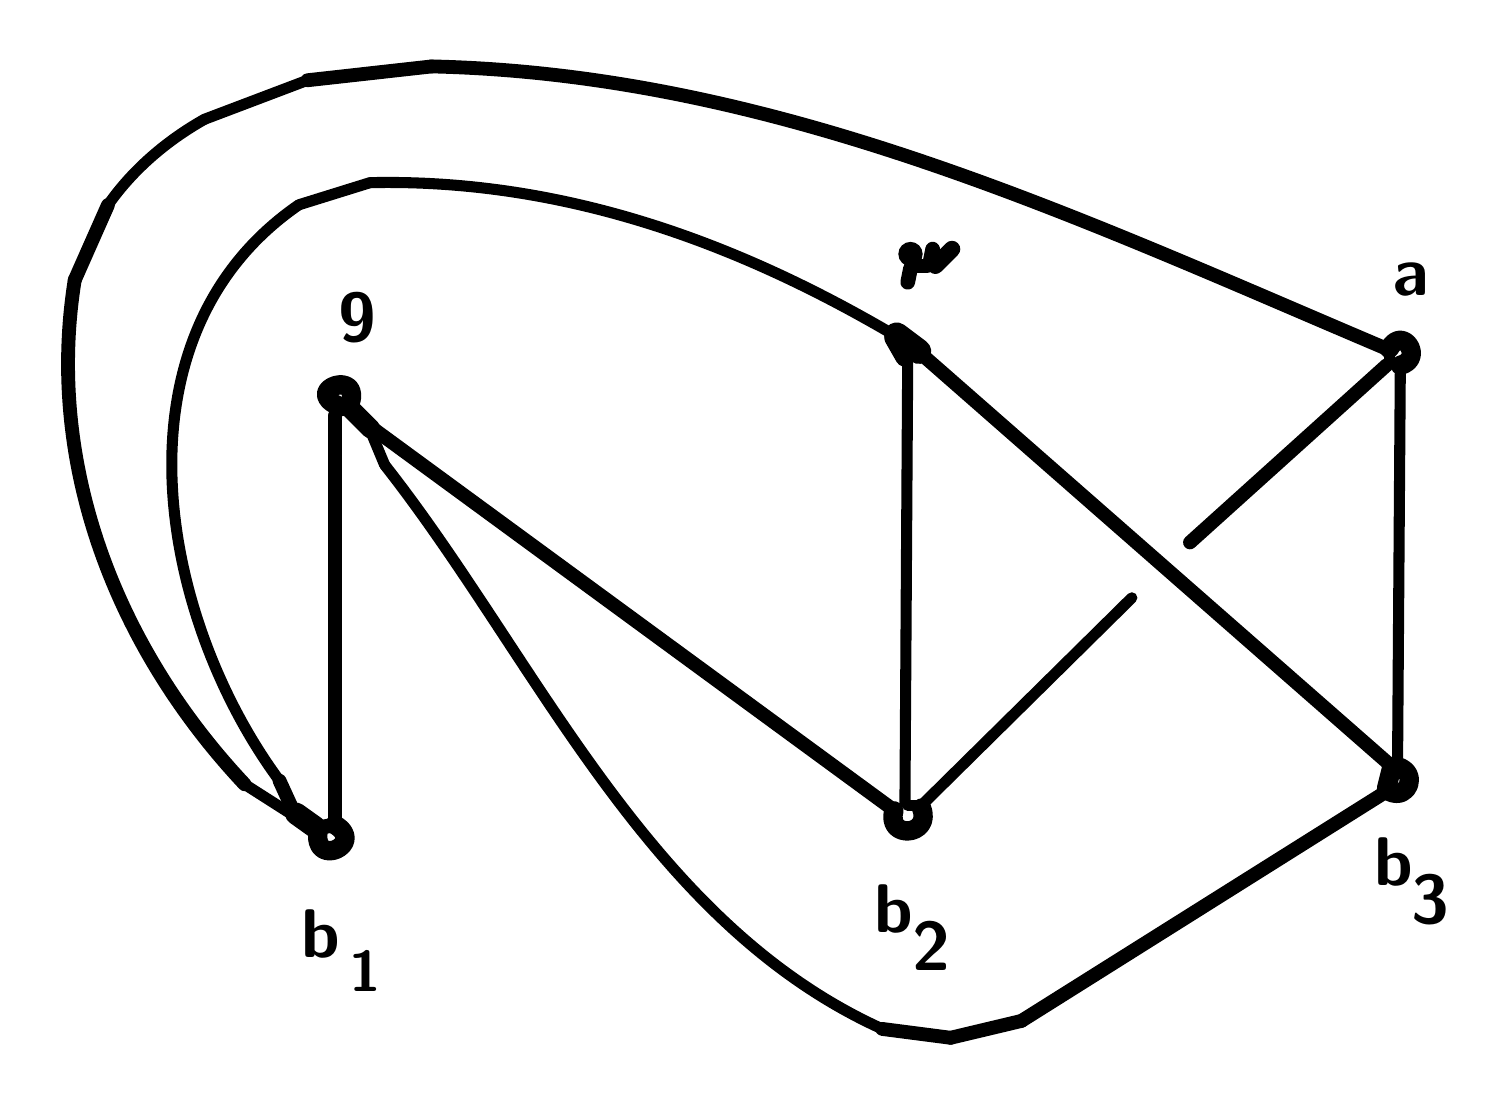
\begin{tikzpicture}[x=1pt, y=-1pt, line width=9.0pt, line cap=round, line join=round]

  %% ════ 填充区（prims2 的 fills）════

  %% ════ 直线段（prims2 的 strokes）════
  \draw[line width=9.0pt] (322.0,117.0) -- (314.0,111.0);
  \draw[line width=4.0pt] (318.0,120.0) -- (317.0,280.0);
  \draw[line width=6.0pt] (328.0,86.0) -- (334.0,80.0);
  \draw[line width=5.0pt] (146.0,14.0) -- (101.1,19.0);
  \draw[line width=4.0pt] (101.1,19.0) -- (63.9,33.1);
  \draw[line width=5.0pt] (29.0,64.1) -- (17.0,91.2);
  \draw[line width=4.0pt] (78.4,273.4) -- (95.0,284.0);
  \draw[line width=5.0pt] (325.0,86.0) -- (320.0,86.0);
  \draw[line width=7.0pt] (124.0,145.0) -- (116.0,137.0);
  \draw[line width=5.3pt] (327.0,80.0) -- (326.0,85.0);
  \draw[line width=5.0pt] (323.0,118.0) -- (493.0,267.0);
  \draw[line width=4.0pt] (323.0,281.0) -- (399.0,206.0);
  \draw[line width=5.0pt] (491.0,122.0) -- (420.0,186.0);
  \draw[line width=4.0pt] (496.0,123.0) -- (495.0,266.0);
  \draw[line width=7.0pt] (313.0,112.0) -- (317.0,119.0);
  \draw[line width=8.0pt] (104.0,289.0) -- (97.0,284.0);
  \draw[line width=5.0pt] (312.0,282.0) -- (125.0,145.0);
  \draw[line width=4.0pt] (492.0,117.0) -- (492.0,121.0);
  \draw[line width=5.0pt] (491.0,276.0) -- (359.1,358.9);
  \draw[line width=5.0pt] (359.1,358.9) -- (333.5,365.0);
  \draw[line width=5.0pt] (333.5,365.0) -- (308.8,361.8);
  \draw[line width=4.0pt] (129.0,158.0) -- (124.0,146.0);
  \draw[line width=3.0pt] (113.0,137.0) -- (116.0,137.0);
  \draw[line width=3.8pt] (113.0,137.0) -- (111.0,140.2);
  \draw[line width=5.0pt] (111.0,140.2) -- (111.0,288.0);
  \draw[line width=4.0pt] (322.0,281.0) -- (318.0,281.0);
  \draw[line width=5.3pt] (106.0,289.0) -- (111.0,288.0);
  \draw[line width=5.0pt] (96.0,283.0) -- (91.0,272.1);
  \draw[line width=4.0pt] (98.0,64.0) -- (123.7,56.0);
  \draw[line width=5.3pt] (319.0,87.0) -- (318.0,92.0);
  \draw[line width=7.0pt] (491.0,275.0) -- (493.0,267.0);

  %% ════ 曲线（prims2 的 curves —— 三段式，坐标同为 (y,x)）════
  \draw[line width=7.0pt] (492.0,276.0) .. controls (498.9,279.4) and (502.7,269.2) .. (495.0,267.0);
  \draw[line width=5.0pt] (491.0,116.0) .. controls (380.3,69.1) and (270.8,16.8) .. (146.0,14.0);
  \draw[line width=4.0pt] (63.9,33.1) .. controls (50.4,40.7) and (38.0,51.2) .. (29.0,64.1);
  \draw[line width=5.0pt] (17.0,91.2) .. controls (6.2,158.5) and (32.5,224.6) .. (78.4,273.4);
  \draw[line width=4.0pt] (308.8,361.8) .. controls (223.3,323.1) and (183.8,227.6) .. (129.0,158.0);
  \draw[line width=7.0pt] (105.0,290.0) .. controls (102.6,304.2) and (122.7,294.9) .. (111.0,288.0);
  \draw[line width=7.0pt] (113.0,137.0) .. controls (97.9,131.0) and (122.2,122.6) .. (116.0,137.0);
  \draw[line width=7.0pt] (313.0,283.0) .. controls (310.1,293.5) and (326.9,292.1) .. (323.0,282.0);
  \draw[line width=7.0pt] (496.0,122.0) .. controls (504.8,119.8) and (496.9,107.3) .. (492.0,116.0);
  \draw[line width=4.0pt] (91.0,272.1) .. controls (47.8,213.7) and (28.4,111.9) .. (98.0,64.0);
  \draw[line width=4.0pt] (123.7,56.0) .. controls (192.9,54.5) and (255.7,77.3) .. (313.0,111.0);

  %% ════ 实心点 ════
  \fill (319.0,81.8) circle (4.4);

  %% ════ 标签（probe 直接给的 \node 行）════
  %% ⚠ 全部补了 fill=white：文字在最上层，否则与曲线交叉干扰
     \node[anchor=center,inner sep=0pt,fill=white,font=\fontsize{32.0}{40.0}\selectfont] at (500.1,91.1) {\textsf{\textbf{\textit{a}}}};   % box(491,81,16,17)
     \node[anchor=center,inner sep=0pt,fill=white,font=\fontsize{34.0}{42.5}\selectfont] at (119.0,104.9) {\textsf{\textbf{9}}};   % box(108,93,18,22)
     \node[anchor=center,inner sep=0pt,fill=white,font=\fontsize{30.0}{37.5}\selectfont] at (493.8,301.2) {\textsf{\textbf{\textit{b}}}};   % box(484,289,17,22)
     \node[anchor=center,inner sep=0pt,fill=white,font=\fontsize{30.0}{37.5}\selectfont] at (312.8,318.2) {\textsf{\textbf{\textit{b}}}};   % box(303,306,17,22)
     \node[anchor=center,inner sep=0pt,fill=white,font=\fontsize{23.0}{28.7}\selectfont] at (506.9,315.1) {\textsf{\textbf{3}}};   % box(501,306,11,17)
     \node[anchor=center,inner sep=0pt,fill=white,font=\fontsize{30.0}{37.5}\selectfont] at (105.8,327.2) {\textsf{\textbf{\textit{b}}}};   % box(96,315,17,22)
     \node[anchor=center,inner sep=0pt,fill=white,font=\fontsize{24.7}{30.9}\selectfont] at (326.6,331.9) {\textsf{\textbf{2}}};   % box(320,323,12,17)
     \node[anchor=center,inner sep=0pt,fill=white,font=\fontsize{21.5}{26.9}\selectfont] at (122.0,340.9) {\textsf{\textbf{1}}};   % box(116,333,7,15)

  % 钉死画布：否则超出的图元/控制点会把页面撑大，1:1 回比就失准
  \pgfresetboundingbox
  \path[use as bounding box] (0,0) rectangle (521,376);
\end{tikzpicture}
\end{document}

% ⚠ 待核清单（probe 拿不准，人眼过一遍）：
%   · 未识别/跳过：⑤ 跳过/未识别的字形
